\textbf{Beispiel 3}\\ \\
a)\\ \\
freigeschnittenes Brett:
\begin{figure}[h]
	\centering
	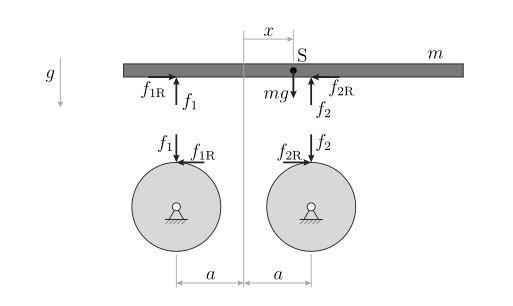
\includegraphics[width= 13cm]{tikz/03_02_2017_3a}
\end{figure}
\newline
Aufgrund der großen Winkelgeschwindigkeit gilt für die trockene Haftreibung immer $\text{sign}(\dot{x}) = 1$ und daraus kann man 
\begin{align*}
	f_{1R} &= \mu_1 f_1 \\
	f_{2R} &= \mu_2 f_2 
\end{align*}
\newpage
\noindent
b)\\ \\
Die Kräfte- und Momentenbilanz für den Balken lautet
\begin{align*}
	f_1 + f_2 - mg &= 0 \\
	-(a + x)f_1 + (a - x)f_2 &= 0
\end{align*}
Aus der ersten der beiden Gleichungen folgt
\[
	f_1 = mg - f_2
\]
Nun wird die zweite Gleichung auf $f_2$ umgeformt.
\[ 
	f_2 = \frac{(a + x)f_1}{a - x}
\]
Setzt man nun diese Gleichung in die erste ein folgt
\begin{align*}
	f_1 &= mg - \frac{(a + x)f_1}{a - x} \\
	f_1(a - x) &= mg(a - x) - (a + x)f_1 \\
	2af_1 &= mg (a - x) \\
	f_1 &= \frac{mg(a - x)}{2a}
\end{align*}
Somit folgt für die andere Normalkraft
\[
	f_2 = \frac{mg (a + x)}{2a}
\]
c)\\ \\
Impulserhaltungssatz
\[
	m\ddot{x} = \mu_1 f_1 - \mu_2 f_2
\]
d)\\ \\
Zuerst setzt man $f_1$ und $f_2$ ein. Dadurch erhält man die Differentialgleichung
\begin{align*}
	m\ddot{x} &= \mu \frac{mg(a - x)}{2a} - \mu\frac{mg (a + x)}{2a} \\
	\ddot{x} &= \mu \frac{g}{2a}(-2x) \\
	\ddot{x} + &\frac{\mu g}{a}x = 0
\end{align*}
Setzt man nun den gegebenen Ansatz in diese Gleichung ein erhält man
\begin{align*}
	\underbrace{\left(-\omega^2 + \frac{\mu g}{a}\right)}_{\overset{!}{=} 0} (A\sin(\omega t) + B\cos(\omega t)) = 0
\end{align*}
Dies führt zur Schwingungskreisfrequenz
\[
	\omega = \sqrt{\frac{\mu g}{a}}
\]
e)\\ \\
Mit den Anfangsbedingungen $x(0) = \dot{x}(0) = 0$ entsteht keine Bewegung beim Brett. \\ \\
f)\\ \\
Mit $\mu_1 \neq \mu_2$ entstehen auch bei x(0) = 0 unterschiedlich große Reibkräfte, welche zu einer resultierenden Kraft für eine Bewegung in x-Richtung führt. Es folgt eine harmonische Schwingung um einen Punkt $x \neq 0$ da mit $\mu_1 \neq \mu_2$ die Symmetrie aufgehoben wird.